\documentclass[11pt,a4paper]{article}
\usepackage[utf8]{inputenc}
\usepackage[T1]{fontenc}
\usepackage{geometry}\geometry{margin=2.5cm}
\usepackage{graphicx,amsmath,amssymb,booktabs,longtable,listings,xcolor,hyperref,float,enumitem,fancyhdr,tikz}
\usetikzlibrary{shapes.geometric,arrows.meta,positioning}

\definecolor{codebg}{RGB}{245,245,245}
\definecolor{codeframe}{RGB}{200,200,200}
\lstset{language=Python,basicstyle=\ttfamily\footnotesize,backgroundcolor=\color{codebg},frame=single,rulecolor=\color{codeframe},breaklines=true,numbers=left,numberstyle=\tiny\color{gray},keywordstyle=\color{blue},commentstyle=\color{green!50!black},stringstyle=\color{red!70!black},showstringspaces=false}

\pagestyle{fancy}\fancyhf{}
\lhead{Gradient-Based Wafer Edge Detection}\rhead{Technical Document}\cfoot{\thepage}

\title{\textbf{Gradient-Based Wafer Edge Detection}\\[4pt]\large Technical Handover Document\\[2pt]\normalsize Wafer Alignment System -- QES (Asia-Pacific) Sdn Bhd}
\author{Engineering Team}\date{May 2026}

\begin{document}
\maketitle\tableofcontents\newpage

% ============================================================
\section{Executive Summary}
This document describes the gradient-based wafer edge detection subsystem. The algorithm finds the precise straight-line boundary of a semiconductor wafer in microscope images, returning sub-pixel edge position and offset from the image centre. It supports four scan directions (LEFT, RIGHT, TOP, BOTTOM), three edge polarity modes, and integrates with the FOV classifier to reject non-edge images.

% ============================================================
\section{Architecture Overview}

\subsection{MVVM Layer Mapping}
\begin{center}
\begin{tabular}{lll}\toprule
\textbf{Layer} & \textbf{File} & \textbf{Role}\\\midrule
Service & \texttt{edge\_finder.py} & Core algorithm (838 lines)\\
Service & \texttt{fov\_classifier.py} & FOV type classification (1418 lines)\\
ViewModel & \texttt{edge\_viewmodel.py} & UI logic, config cache\\
View & \texttt{edge\_tab.py} & Tkinter widgets\\
Model & \texttt{recipe\_model.py} & XML recipe persistence\\
Model & \texttt{app\_state.py} & Per-direction config cache\\
Integration & \texttt{zmq\_server.py} & ZeroMQ TCP interface\\\bottomrule
\end{tabular}
\end{center}

\subsection{Dependency Graph}
\begin{center}
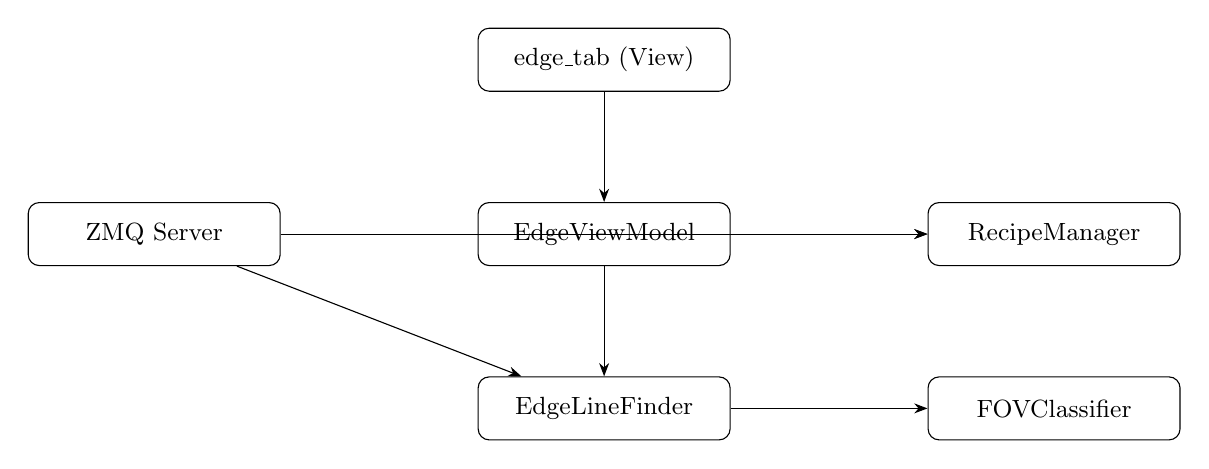
\begin{tikzpicture}[node distance=1.4cm,every node/.style={draw,rounded corners,minimum width=3.2cm,minimum height=0.8cm,font=\small}]
\node(V){edge\_tab (View)};
\node(VM)[below=of V]{EdgeViewModel};
\node(EF)[below=of VM]{EdgeLineFinder};
\node(FOV)[right=2.5cm of EF]{FOVClassifier};
\node(R)[right=2.5cm of VM]{RecipeManager};
\node(Z)[left=2.5cm of VM]{ZMQ Server};
\draw[-{Stealth}](V)--(VM);
\draw[-{Stealth}](VM)--(EF);
\draw[-{Stealth}](EF)--(FOV);
\draw[-{Stealth}](VM)--(R);
\draw[-{Stealth}](Z)--(EF);
\draw[-{Stealth}](Z)--(R);
\end{tikzpicture}
\end{center}

% ============================================================
\section{Algorithm Pipeline}

\begin{center}
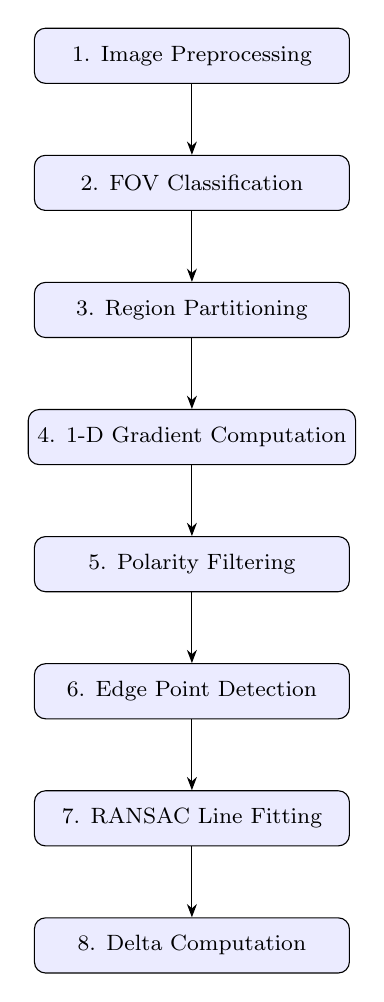
\begin{tikzpicture}[node distance=0.9cm,every node/.style={draw,rounded corners,minimum width=4cm,minimum height=0.7cm,font=\footnotesize,fill=blue!8}]
\node(A){1. Image Preprocessing};
\node(B)[below=of A]{2. FOV Classification};
\node(C)[below=of B]{3. Region Partitioning};
\node(D)[below=of C]{4. 1-D Gradient Computation};
\node(E)[below=of D]{5. Polarity Filtering};
\node(F)[below=of E]{6. Edge Point Detection};
\node(G)[below=of F]{7. RANSAC Line Fitting};
\node(H)[below=of G]{8. Delta Computation};
\draw[-{Stealth}](A)--(B);\draw[-{Stealth}](B)--(C);\draw[-{Stealth}](C)--(D);
\draw[-{Stealth}](D)--(E);\draw[-{Stealth}](E)--(F);\draw[-{Stealth}](F)--(G);\draw[-{Stealth}](G)--(H);
\end{tikzpicture}
\end{center}

% ============================================================
\section{Detailed Algorithm Description}

\subsection{Step 1: Image Preprocessing}
\textbf{Function}: \texttt{preprocess\_image(img\_or\_path, target\_dim)}

\begin{enumerate}
\item Load image as grayscale (\texttt{cv2.imread} with flag 0).
\item Resize so the longest dimension equals \texttt{TARGET\_PROCESS\_DIM} (default 1000\,px). Record scale factor $s = 1000 / \max(H,W)$.
\item Apply CLAHE (Contrast Limited Adaptive Histogram Equalisation): \texttt{clipLimit=2.0}, \texttt{tileGridSize=8$\times$8}.
\end{enumerate}

The scale factor $s$ is used later to convert detected coordinates back to original-resolution pixels.

\subsection{Step 2: FOV Classification}
\textbf{Class}: \texttt{FOVClassifier} (in \texttt{fov\_classifier.py})

Determines if the image contains a wafer edge (\texttt{EDGE\_FOV}), die patterns (\texttt{DIE\_FOV}), or plain wafer surface (\texttt{WAFER\_FOV}). This step is skipped when \texttt{skip\_classification=True} (param tuner mode or ZMQ \texttt{FORCE\_RUN}).

Classification uses four parallel detectors:
\begin{enumerate}
\item \textbf{1-D Edge Detection}: Horizontal and vertical intensity profiles from 4 bands. Detects monotonic rising/falling regions with adaptive thresholds (percentile-based).
\item \textbf{2-D Sobel Edge Detection}: Downsampled $4\times$, Sobel gradients, checks if strong gradients are spatially concentrated (edge) vs distributed (die).
\item \textbf{Peak-Based Classifier}: Counts prominent peaks in 1-D projections. $\leq 2$ peaks $\rightarrow$ edge; $\geq 5$ $\rightarrow$ die.
\item \textbf{Region Analysis}: Splits image into 6 regions (left/centre/right $\times$ top/centre/bottom). Classifies each by texture score (Laplacian variance) and gradient peak count.
\end{enumerate}

Confidence score (0--1) computed from signal strength, region consistency, and detector agreement. Below \texttt{CONFIDENCE\_THRESHOLD} (0.40) $\rightarrow$ \texttt{UNCERTAIN}.

\subsection{Step 3: Region Partitioning}
The image is divided into \texttt{NUM\_REGIONS} (default 40) horizontal or vertical strips:

\begin{itemize}
\item \textbf{LEFT/RIGHT} (vertical edge): $N$ horizontal strips, each of height $H/N$. Each strip produces one edge point along the $x$-axis.
\item \textbf{TOP/BOTTOM} (horizontal edge): $N$ vertical strips, each of width $W/N$. Each strip produces one edge point along the $y$-axis.
\end{itemize}

\subsection{Step 4: 1-D Gradient Computation}
For each region strip:
\begin{enumerate}
\item Compute the \textbf{median intensity profile} along the scan axis. Median is used instead of mean for robustness against outlier pixels.
\item Convolve with a gradient kernel: $K = [-1, \ldots, -1, 0, 1, \ldots, 1]$ of size \texttt{KERNEL\_SIZE} (default 7).
\end{enumerate}

\paragraph{Gradient Kernel Construction}
\textbf{Function}: \texttt{create\_gradient\_kernel(size)}
\begin{lstlisting}
# size=7 -> [-1, -1, -1, 0, 1, 1, 1]
kernel = np.concatenate([-np.ones(half), np.zeros(1), np.ones(half)])
\end{lstlisting}
Multiple $-1$/$+1$ elements improve noise resistance compared to a simple $[-1, 0, 1]$ kernel.

\subsection{Step 5: Edge Polarity Filtering}
\textbf{Function}: \texttt{\_apply\_polarity(gradient)}

Three modes:
\begin{center}
\begin{tabular}{lp{9cm}}\toprule
\textbf{Mode} & \textbf{Behaviour}\\\midrule
\texttt{ANY} & No filtering; detect edges of any polarity\\
\texttt{LIGHT\_TO\_DARK} & Zero out positive gradient values (keep only bright$\rightarrow$dark transitions)\\
\texttt{DARK\_TO\_LIGHT} & Zero out negative gradient values (keep only dark$\rightarrow$bright transitions)\\\bottomrule
\end{tabular}
\end{center}

\textbf{Direction compensation}: For LEFT and TOP scan directions, the gradient kernel's intrinsic direction is opposite to the conceptual scan direction, so the polarity interpretation is flipped. This ensures ``Light-to-Dark'' always means ``bright on the approach side'' regardless of scan direction.

\subsection{Step 6: Edge Point Detection}
\textbf{Functions}: \texttt{\_detect\_edge\_point\_horizontal} / \texttt{\_detect\_edge\_point\_vertical}

\begin{enumerate}
\item Apply border ignore: zero out gradient values within \texttt{BORDER\_IGNORE\_PCT} (default 2\%) of image edges.
\item Find indices where $|\text{gradient}| > \texttt{EDGE\_THRESHOLD}$ (default 25).
\item \textbf{Cluster Analysis}: Identify contiguous clusters separated by gaps $>$ \texttt{MAX\_CLUSTER\_GAP} (default 5 pixels).
\item \textbf{Cluster Selection}: Based on scan direction:
  \begin{itemize}
  \item LEFT: first cluster from left (edge is on the left side)
  \item RIGHT: last cluster from left
  \item TOP: first cluster from top
  \item BOTTOM: last cluster from bottom
  \end{itemize}
\item Find the peak within the selected cluster: $\arg\max |\text{gradient}|$.
\item \textbf{Sub-pixel refinement} via 3-point parabolic fit:
\[
x_\text{sub} = x_\text{peak} + \frac{g[x_\text{peak}-1] - g[x_\text{peak}+1]}{2\bigl(g[x_\text{peak}-1] - 2g[x_\text{peak}] + g[x_\text{peak}+1]\bigr)}
\]
Offset clamped to $[-0.5, +0.5]$.
\item The $y$-coordinate is the centre of the region strip.
\end{enumerate}

\subsection{Step 7: RANSAC Line Fitting}
\textbf{Function}: \texttt{fit\_line\_ransac(points, iterations, threshold)}

\begin{enumerate}
\item Requires $\geq 3$ detected points.
\item For \texttt{RANSAC\_ITERATIONS} (default 2000) iterations:
  \begin{enumerate}
  \item Randomly sample 2 points.
  \item Compute line $Ax + By + C = 0$.
  \item Count inliers: points with perpendicular distance $< \texttt{RANSAC\_THRESHOLD}$ (default 5.0\,px).
  \item Keep the model with the most inliers.
  \end{enumerate}
\item Refine with \texttt{cv2.fitLine} (L2 distance) on the inlier set.
\item Extract direction vector $(v_x, v_y)$, point $(x_0, y_0)$, and compute line endpoints at image boundaries.
\end{enumerate}

\paragraph{Line Equation}
The general form $Ax + By + C = 0$ is computed as:
\[A = v_y, \quad B = -v_x, \quad C = -v_y \cdot x_0 + v_x \cdot y_0\]

\subsection{Step 8: Perpendicular Delta Computation}
\textbf{Function}: \texttt{compute\_perpendicular\_delta(A, B, C, img\_h, img\_w, scale)}

Matches the C\# \texttt{EmguVision.cs} implementation (WEPLEFT\_REQ lines 776--787):
\begin{enumerate}
\item Image centre in downsampled space: $(c_x, c_y) = (W/2, H/2)$.
\item Foot of perpendicular from centre to line:
\[
t = \frac{Ac_x + Bc_y + C}{A^2 + B^2}, \quad p_x = c_x - At, \quad p_y = c_y - Bt
\]
\item Convert to original-resolution pixels: $p_x^\text{orig} = p_x / s$, $p_y^\text{orig} = p_y / s$.
\item Delta: $\Delta x = p_x^\text{orig} - c_x^\text{orig}$, $\Delta y = p_y^\text{orig} - c_y^\text{orig}$.
\end{enumerate}

These deltas represent the offset of the wafer edge from the camera's optical centre, which the motion controller uses to align the wafer.

% ============================================================
\section{Configuration Reference}

\begin{longtable}{p{4.2cm}p{2.2cm}p{7cm}}\toprule
\textbf{Parameter} & \textbf{Default} & \textbf{Description}\\\midrule\endhead
\texttt{SCAN\_DIRECTION} & LEFT & Edge side: LEFT, RIGHT, TOP, BOTTOM\\
\texttt{EDGE\_POLARITY} & ANY & Polarity filter: ANY, LIGHT\_TO\_DARK, DARK\_TO\_LIGHT\\
\texttt{NUM\_REGIONS} & 40 & Number of scan strips\\
\texttt{EDGE\_THRESHOLD} & 25 & Minimum gradient magnitude for edge\\
\texttt{MAX\_CLUSTER\_GAP} & 5 & Max gap between cluster points (px)\\
\texttt{BORDER\_IGNORE\_PCT} & 0.02 & Image border exclusion zone (2\%)\\
\texttt{RANSAC\_ITERATIONS} & 2000 & RANSAC iteration count\\
\texttt{RANSAC\_THRESHOLD} & 5.0 & Inlier distance threshold (px)\\
\texttt{KERNEL\_SIZE} & 7 & Gradient kernel width (odd, $\geq 3$)\\
\texttt{TARGET\_PROCESS\_DIM} & 1000 & Resize target for processing\\
\texttt{CLAHE\_CLIP\_LIMIT} & 2.0 & CLAHE clip limit (0=off)\\
\texttt{CLAHE\_GRID\_SIZE} & 8 & CLAHE tile grid size\\\bottomrule
\end{longtable}

% ============================================================
\section{Data Structures}

\subsection{EdgeFinderConfig}
Extends \texttt{ClassificationConfig}. All edge-specific parameters listed in \S5 plus inherited FOV classification settings.

\subsection{find\_edge() Return Dict}
\begin{lstlisting}
{
  'success': bool,
  'line_params': {'a':float,'b':float,'c':float,
                  'vx':float,'vy':float,'x0':float,'y0':float},
  'line_endpoints': {'x_top':int,'x_bot':int}  # or y_left,y_right
  'slope': float,
  'intercept_c': float,
  'delta_x': float,       # original-resolution offset
  'delta_y': float,
  'intercept_point': {'x':float, 'y':float},
  'detected_points': [(x,y), ...],
  'inliers': np.array,
  'num_points': int,
  'num_inliers': int,
  'region_data': [{'region_start':int, 'region_end':int,
                   'profile':np.array, 'gradient':np.array,
                   'edge_point':dict}, ...],
  'image': np.array,       # processed image
  'original_image': np.array,
  'scale': float,
  'scan_direction': str,
  'is_vertical_edge': bool,
  'reason': str or None
}
\end{lstlisting}

% ============================================================
\section{ZMQ Integration}

\subsection{WAFER\_EDGE\_REQ Command}
\begin{verbatim}
WAFER_EDGE_REQ "<image_path>" "<recipe_path>" <direction>
               [<polarity>] [FORCE_RUN]
\end{verbatim}

\textbf{Parameters}:
\begin{itemize}[nosep]
\item \texttt{image\_path}: Full path to the image to analyse.
\item \texttt{recipe\_path}: Recipe XML (name or full path).
\item \texttt{direction}: LEFT $|$ RIGHT $|$ TOP $|$ BOTTOM.
\item \texttt{polarity}: (optional) ANY $|$ LIGHT\_TO\_DARK $|$ DARK\_TO\_LIGHT.
\item \texttt{FORCE\_RUN}: (optional) Skip FOV classification.
\end{itemize}

\textbf{Response variants}:
\begin{lstlisting}[language={}]
{"status":"ok", "delta_x":-123.4, "delta_y":5.6,
 "fov_type":"EDGE_FOV", "fov_confidence":0.95,
 "a":..., "b":..., "c":..., "x_top":..., "x_bot":...}

{"status":"die_fov_warning", "fov_type":"DIE_FOV",
 "message":"Resend with FORCE_RUN to override."}

{"status":"no_edge", "reason":"Not enough points"}
\end{lstlisting}

\subsection{DIE\_FOV Warning Flow}
\begin{enumerate}
\item C\# sends \texttt{WAFER\_EDGE\_REQ} without \texttt{FORCE\_RUN}.
\item If FOV classifier returns \texttt{DIE\_FOV}, Python replies with \texttt{die\_fov\_warning}.
\item C\# shows a dialog to the operator.
\item If operator confirms, C\# resends with \texttt{FORCE\_RUN} appended.
\item Python runs edge detection regardless of FOV type.
\end{enumerate}

% ============================================================
\section{Recipe XML Schema (FindWaferEdge)}
\begin{lstlisting}[language=XML]
<FindWaferEdge>
  <UseUniversalParams>false</UseUniversalParams>
  <WaferAlignLeftParam Name="Wafer Align Left Parm">
    <KernelSize>9</KernelSize>
    <EdgeThreshold>500</EdgeThreshold>
    <NumRegions>30</NumRegions>
    <BorderIgnorePct>0.05</BorderIgnorePct>
    <RansacThreshold>3.0</RansacThreshold>
    <EdgePolarity>ANY</EdgePolarity>
  </WaferAlignLeftParam>
  <!-- WaferAlignRightParam, WaferAlignTopParam,
       WaferAlignBotParam follow same structure -->
</FindWaferEdge>
\end{lstlisting}

Each scan direction has independent parameter sets. The \texttt{UseUniversalParams} flag (when true) applies LEFT parameters to all directions.

% ============================================================
\section{Per-Direction Config Caching}

The \texttt{AppState} maintains a dict \texttt{edge\_configs} with keys LEFT/RIGHT/TOP/BOTTOM. When the user switches the direction dropdown:
\begin{enumerate}
\item \texttt{EdgeViewModel.save\_current\_dir\_to\_cache(old\_dir)} saves current slider values.
\item \texttt{EdgeViewModel.get\_cache\_for\_dir(new\_dir)} loads cached values for the new direction.
\item The View updates slider positions without triggering detection.
\end{enumerate}

% ============================================================
\section{Visualisation}

The \texttt{EdgeLineFinder.visualize()} method produces a 4-panel Matplotlib figure:
\begin{enumerate}
\item \textbf{Result Image}: Detected line (green), all detected points (red circles), RANSAC inliers (yellow circles).
\item \textbf{Gradient Profile}: 1-D gradient of the middle region with threshold line and peak marker.
\item \textbf{Point Scatter}: All detected points vs fitted line, with inliers highlighted.
\item \textbf{Summary Panel}: Status, point counts, line endpoints, angle.
\end{enumerate}

The \texttt{EdgeViewModel.compute\_gradient\_display()} method produces:
\begin{itemize}
\item 2-D gradient magnitude image with HOT colourmap overlay.
\item 1-D gradient profile for the Matplotlib graph in the Edge tab.
\end{itemize}

% ============================================================
\section{FOV Classifier Details}

\subsection{Classification Config}
\begin{longtable}{p{4.8cm}p{1.8cm}p{7cm}}\toprule
\textbf{Parameter} & \textbf{Default} & \textbf{Description}\\\midrule\endhead
\texttt{RELATIVE\_CHANGE\_WEAK} & 0.15 & 15\% of dynamic range for weak edge\\
\texttt{RELATIVE\_CHANGE\_STRONG} & 0.25 & 25\% for strong edge\\
\texttt{MIN\_INTENSITY\_CHANGE\_WEAK} & 30 & Absolute fallback threshold\\
\texttt{MIN\_INTENSITY\_CHANGE\_STRONG} & 50 & Absolute fallback threshold\\
\texttt{MIN\_LENGTH\_RATIO\_LONG} & 0.15 & Minimum monotonic region length\\
\texttt{MIN\_LENGTH\_RATIO\_SHORT} & 0.05 & Minimum for sharp edges\\
\texttt{SOBEL\_STRENGTH\_THRESHOLD} & 0.20 & 2-D Sobel edge threshold\\
\texttt{CONFIDENCE\_THRESHOLD} & 0.40 & Below this $\rightarrow$ UNCERTAIN\\
\texttt{DIE\_OVERRIDE\_PCT} & 100 & \% regions that must be DIE to override\\\bottomrule
\end{longtable}

\subsection{1-D Edge Detection Criteria}
Five criteria checked in order (first match wins):
\begin{enumerate}
\item \textbf{Curved Rising}: Long monotonic rise ($\geq 15\%$ of profile), weak threshold, not periodic.
\item \textbf{Curved Falling}: Same for falling.
\item \textbf{Sharp Rising}: Short rise ($\geq 5\%$), strong threshold, not periodic.
\item \textbf{Sharp Falling}: Same for falling.
\item \textbf{Quarter Difference}: First-quarter vs last-quarter mean intensity difference exceeds threshold.
\end{enumerate}

% ============================================================
\section{C\# Compatibility Notes}

\begin{itemize}
\item \textbf{Delta calculation} matches \texttt{EmguVision.cs} lines 776--787 (perpendicular-intersection method).
\item \textbf{ZMQ protocol} uses the same command format as the C\# \texttt{VPServer} process commands.
\item \textbf{Recipe XML} schema matches the C\# \texttt{WaferAlignLeftParam} / \texttt{WaferAlignRightParam} / etc.\ structure.
\item Direction-specific parameter storage mirrors C\# per-side settings.
\end{itemize}

% ============================================================
\section{Known Limitations \& Future Work}
\begin{itemize}
\item Curved wafer edges (large FOV) may produce slightly non-linear edge lines; a polynomial fit could improve accuracy.
\item The FOV classifier occasionally misclassifies strong die patterns near the wafer edge as \texttt{EDGE\_FOV}.
\item Gradient kernel is fixed; adaptive kernel selection based on image noise could improve robustness.
\item No GPU acceleration (edge detection is fast enough on CPU at $\sim$50\,ms for 1000\,px processed images).
\end{itemize}

% ============================================================
\section{File Reference}
\begin{longtable}{p{5.5cm}p{8cm}}\toprule
\textbf{File} & \textbf{Purpose}\\\midrule
\texttt{app/services/edge\_finder.py} & Core edge detection algorithm (838 lines)\\
\texttt{app/services/fov\_classifier.py} & FOV classification (1418 lines)\\
\texttt{app/viewmodels/edge\_viewmodel.py} & UI business logic, config caching (208 lines)\\
\texttt{app/views/edge\_tab.py} & Tkinter tab UI\\
\texttt{app/models/recipe\_model.py} & XML recipe read/write\\
\texttt{app/models/app\_state.py} & Per-direction config cache\\
\texttt{app/services/zmq\_server.py} & ZMQ server (WAFER\_EDGE\_REQ handler)\\\bottomrule
\end{longtable}

\end{document}
